\chapter{Input of \software{echse}-based models} \label{chap:input}
\renewcommand{\tabdir}{chapters/input/tab}
\renewcommand{\figdir}{chapters/input/fig}

%%%%%%%%%%%%%%%%%%%%%%%%%%%%%%%%%%%%%%%%%%%%%%%%%%%%%%%%%%%%%%%%%%%%%%%%%%%%%%%%
%%%%%%%%%%%%%%%%%%%%%%%%%%%%%%%%%%%%%%%%%%%%%%%%%%%%%%%%%%%%%%%%%%%%%%%%%%%%%%%%
%%%%%%%%%%%%%%%%%%%%%%%%%%%%%%%%%%%%%%%%%%%%%%%%%%%%%%%%%%%%%%%%%%%%%%%%%%%%%%%%
\section{Mandatory command line arguments} \label{sec:input-commandline}

Some basic settings are passed to the model via the command line\index{command line}. Each of these settings is identified by a unique keyword. The keyword must be followed by the equal sign '=', followed by a corresponding value. There must be no spaces before or after the equal sign. The expected keyword-value pairs are summarized in \tabref{tab:input-commandline}. They may appear at the command line in any order. In addition to these mandatory arguments, further configuration data may be passed via the command line (see \secref{sec:input-config}).

\begin{table*}
  \caption{Mandatory command line arguments of a model. \label{tab:input-commandline}}
  \begin{tabular}{p{0.17\textwidth}p{0.1\textwidth}p{0.63\textwidth}} \hline
    \textbf{Keyword} & \textbf{Data type} & \textbf{Description} \\ \hline
    \verb!file_control! & string &
      Name/path of the configuration file. This file contains all configuration data (except for those data specified as additional command line arguments). The configuration data are discussed in detail in \secref{sec:input-config}. \\
    \verb!file_log! & string &
      Name/path of the log file created during a model run. The log file contains a compact documentation of all major steps of processing. Its contents is usually inspected in the case of abnormal program termination. \\
    \verb!file_err! & string &
      Name/path of a file where traceback information should be written to. This file will only be generated if the model terminates after occurrence of an exception. In the vast majority of cases, the information found in this file will help to quickly identify what caused the exception. \\
    \verb!format_err! & string &
      This option controls the format used in the file specified as \verb!file_err!.  The supported codes currently include 'xml', 'html', and 'txt'. For visual inspection, the html-format is the preferred choice. The other formats are more useful for automatic extraction of information (if the model is running in a more complex software environment, for example). If an unsupported format code is supplied, the 'txt' format will be used. \\
    \verb!silent! & logical &
      The model sends basic messages about the current state of processing to standard output (usually the screen) if \verb!silent=false!. This kind of output may be suppressed by setting \verb!silent=true!.\\
    \hline
  \end{tabular}
\end{table*}

A typical call of the model in a shell script using only the mandatory arguments might look as follows:

\texttt{model \textbf{file\_control}=config.txt \textbf{file\_log}=log.txt \textbf{file\_err}=err.html \textbf{format\_err}=html \textbf{silent}=false}

%%%%%%%%%%%%%%%%%%%%%%%%%%%%%%%%%%%%%%%%%%%%%%%%%%%%%%%%%%%%%%%%%%%%%%%%%%%%%%%%
%%%%%%%%%%%%%%%%%%%%%%%%%%%%%%%%%%%%%%%%%%%%%%%%%%%%%%%%%%%%%%%%%%%%%%%%%%%%%%%%
%%%%%%%%%%%%%%%%%%%%%%%%%%%%%%%%%%%%%%%%%%%%%%%%%%%%%%%%%%%%%%%%%%%%%%%%%%%%%%%%
\section{General notes on file formats} \label{sec:input-formats}

All input files comply with a simple quasi-standard\index{format!files} and can easily be created automatically (by scripts or any spreadsheet software). For small projects, the files can even be created manually using just a text editor. The general rules applying to all input files are as follows:
\begin{description}
  \item [Tabular format] All input files actually represent tables. The number of columns varies from file to file and the number of rows (records) depends generally on the particular application. The number of columns must be consistent for all records. The tables are in plain text format.
  \item [Column separator] The table columns are separated by a reserved character which has to be specified in the configuration file (see \secref{sec:input-config}). Recommended choices are the TAB-character (ASCII code 9), and/or the blank character, or the semi-colon (quasi-standards). As an exception to the above, the column separator used in the configuration file is the equal sign ('=') and it cannot be altered by the user.
  \item [Table header] The first non-blank, non-comment line of a file is interpreted as the table header contaning column names. Tables without header are not supported.
  \item [Character set] An input file should contain nothing but ASCII characters. Other characters may or may not be interpreted correctly (to be tested).
  \item [Comment lines] Comment character(s) have to be be specified in the configuration file (see \secref{sec:input-config}). A line starting with one of the selected comment characters is ignored when reading the table.
  \item [Blank lines] Blank lines are ignored when reading the table, just like comment lines.
  \item [Platform independency] Line endings may be system specific. On Linux/unix, the standard is \verb!\n!. On Windows, it is \verb!\r\n!. Input files prepared for Linux usually also work on Windows and vice-versa (to be tested). The line endings in the output files depend on the platform on which the model is running (see standards above).
  \item [Order of columns] With one exception, the columns of a table can be in any order (since they are identified by the columns' names). The only exception are time series data files (see \secref{sec:input-timeseries}), where the time information must be in the first column. Subsequent columns (containing data values for different locations or variables) may be in any order.
  \item [Column types] The supported data types of a column are: string, integer, numeric, logical, and datetime. For numerical values the usual f-format (0.1) or the scientific e-format (1.e-01) may be used. Valid logical values are \true{} and \false{} (not case-sensitive). Datetime values must be strings in ISO 8601 format\index{format!datetime}, i.e.{} in format \texttt{YYYY-MM-DD hh:mm:ss}. Date and time must be separated by a single character (recommended is a blank).
  \item [File names] Some tables contain references to other files. A file name can be specified using either the absolute or relative path.
  \item [Empty tables] There are no optional input files, which means that all files must exist and must be readable, even if they are not required for a particular application. Even if there is no information to be filled in, you cannot just supply an empty file. Instead you must supply a proper table with the usual header line and (at least) one record of values. The values may (and should be) dummy values that are easily identified as dummies. This procedure may seem overly complicated at first but, in fact, it avoids many other problems (tests in the source code, documentation of optional files, etc.).
\end{description}

%%%%%%%%%%%%%%%%%%%%%%%%%%%%%%%%%%%%%%%%%%%%%%%%%%%%%%%%%%%%%%%%%%%%%%%%%%%%%%%%
%%%%%%%%%%%%%%%%%%%%%%%%%%%%%%%%%%%%%%%%%%%%%%%%%%%%%%%%%%%%%%%%%%%%%%%%%%%%%%%%
%%%%%%%%%%%%%%%%%%%%%%%%%%%%%%%%%%%%%%%%%%%%%%%%%%%%%%%%%%%%%%%%%%%%%%%%%%%%%%%%
\section{Units of variables and constants} \label{sec:input-units}

There is no general convention, \ie{} arbitrary units\index{units} may be used for all constants and variables. The only important facts are:
\begin{itemize}
  \item The units of all variables and constants used in any equations must be consistent. There are no (and cannot be) any built-in checks in the generic part of the source code.
  \item The length of a modeling time step passed to the classes' simulate methods as argument \verb!delta_t! is given in units of seconds.
\end{itemize}

\FloatBarrier

%%%%%%%%%%%%%%%%%%%%%%%%%%%%%%%%%%%%%%%%%%%%%%%%%%%%%%%%%%%%%%%%%%%%%%%%%%%%%%%%
%%%%%%%%%%%%%%%%%%%%%%%%%%%%%%%%%%%%%%%%%%%%%%%%%%%%%%%%%%%%%%%%%%%%%%%%%%%%%%%%
%%%%%%%%%%%%%%%%%%%%%%%%%%%%%%%%%%%%%%%%%%%%%%%%%%%%%%%%%%%%%%%%%%%%%%%%%%%%%%%%
\section{Configuration data} \label{sec:input-config}

%%%%%%%%%%%%%%%%%%%%%%%%%%%%%%%%%%%%%%%%%%%%%%%%%%%%%%%%%%%%%%%%%%%%%%%%%%%%%%
\subsection{Alternative ways of passing config data} \label{sec:input-config-passing}
The configuration data \index{configuration data} comprise all information about a specific model run. This includes, for example, settings like the start and end time of the simulation or the names of the various files which have to be read before or during a model run. The actual data contained in the referenced files (such as time series of external forcings, parameter values, etc.), by definition, do \emph{not} belong to the configuration data.

There are two ways of passing configuration data to the model:
\begin{itemize}
  \item via a configuration file.
  \item via the command line, in addition to the mandatory arguments introduced in \secref{sec:input-commandline}.
\end{itemize}

%%%%%%%%%%%%%%%%%%%%%%%%%%%%%%%%%%%%%%%%%%%%%%%%%%%%%%%%%%%%%%%%%%%%%%%%%%%%%%
\subsection{Syntax conventions} \label{sec:input-config-syntax}
A single configuration data item generally consists of two parts: A keyword and a corresponding value. The general syntax is shown in the following example:

\medskip
\begin{verbatim}
  fruit=apple
  number=22
  apple_data=/home/fred/apples.txt
\end{verbatim}
\medskip

Thus, the keyword must be followed by the equal sign ('='), followed by the value. The value may be a string, a number, a logical value, or a string encoding a datetime value (see \secref{sec:input-formats}). To avoid ambiguities, one cannot pass the same configuration data item (identified by its keyword) via the command line \emph{and} via the configuration file. Multiple definitions of the same keyword are generally considered as errors. The configuration data items may appear in any order. This applies to both the configuration file and the command line.

It is important to note that blank(s) right before the '=' character as in \texttt{key~=value} are \emph{not} allowed (since the blank would be treated as part of the keyword). Some care is necessary if blanks or special characters appear \emph{after} the '=' character . Here are the rules:

If the configuration data item is defined in the configuration file, all blanks after the '=' are treated as part of the value string. You don't need to use quotes here. Typical examples are shown below:
\begin{verbatim}
  item1=2012-01-19 00:00:00
  item2=c:\my files\data.txt
\end{verbatim}

If a configuration data item containing blanks should be passed via the command line, quotes must be used as in the subsequent example, where \verb!*! stands for the mandatory arguments (see \secref{sec:input-commandline}). Blank(s) must not appear between the '=' character and the opening quotes.
\begin{verbatim}
  model * date="2012-01-19 00:00:00"
\end{verbatim}

If a configuration data item contains special characters, it must not be specified at the command line but needs to be defined in the configuration file. This is due to the fact that those characters may be dropped by the C++ command line interpreter. A prominent example is the TAB character (ASCII code 9).

%%%%%%%%%%%%%%%%%%%%%%%%%%%%%%%%%%%%%%%%%%%%%%%%%%%%%%%%%%%%%%%%%%%%%%%%%%%%%%
\subsection{Indirect file references} \label{sec:input-config-indirectRef}
The configuration data usually contain both \emph{direct} and \emph{indirect file references}. Since the latter are sometimes confusing to users, the difference between the two types of file references is briefly discussed. 

\paragraph{A \emph{direct} reference} is present if a configuration data item points to a \emph{data file} containing anything but file names (typically numbers and possibly some alphanumeric IDs). What happens internally is this:
\begin{itemize}
  \item The model engine reads the configration item and finds the reference to a data file 'A'.
  \item At the approriate stage of processing, the model engine reads the data from 'A'.
\end{itemize}

\paragraph{An \emph{indirect} reference} is present if a configuration data item points to a file which contains references to further files. What happens internally is this:
\begin{itemize}
  \item The model engine reads the configration item and finds the reference to a file 'A'.
  \item The model reads file 'A' and finds references to the files 'B' and 'C'.
  \item At the approriate stage of processing, the model engine reads the data from 'B' and 'C'.
\end{itemize}

In theory, it would be possible to use a cascade of such indirect references. The current version of the \software{echse}, however, uses indirect references of the first level only. See \secsref{sec:input-externalVariables}, \ref{sec:input-indivParamFun} \& \ref{sec:input-sharedParamFun} for examples.

%%%%%%%%%%%%%%%%%%%%%%%%%%%%%%%%%%%%%%%%%%%%%%%%%%%%%%%%%%%%%%%%%%%%%%%%%%%%%%
\subsection{Overview of configuration data items} \label{sec:input-config-items}
The various configuration data items expected by an \software{echse}-based model are described in detail \tabsref{tab:config-compuational} -- \ref{tab:config-params}.

\begin{table*}
  \caption{Keywords of the configuration file controlling the computational behavior. \label{tab:config-compuational}}
\begin{tabular}{p{0.32\textwidth}p{0.1\textwidth}p{0.48\textwidth}} \hline
\textbf{Keyword} & \textbf{Data type} & \textbf{Description} \\ \hline
\verb!trap_fpe! & logical &
  If \true{} (recommended), an exception will be thrown if invalid floating point numbers occur in an object's state or output variables. If \false{}, the computation continues (if possible) and \texttt{NaN} or \texttt{Inf} values may appear in output files. \\
\verb!number_of_threads! & integer & The desired number of threads to be run in parallel. Values greater than one will only have an effect on multi-core machines. If the requested number exceeds the maximum possible number of threads on the particular machine, the possible maximum is used. See also keyword \verb!singlethread_if_less_than! and consult \secref{sec:guidelines-speedOptim-parallel} before setting \verb!number_of_threads! to a value greater than 1. \\
\verb!singlethread_if_less_than! & integer &
  This key lets you define a threshold value for parallel processing. If the number of objects of a particular level is $<$ this threshold, these objects will be simulated by a single thread (\ie{} in serial mode) even if parallel processing was requested by the keyword \verb!number_of_threads!. If the number of objects of a particular level is $geq$ this threshold, the requested (or possible) number of threads will be used. \\
\hline
\end{tabular}
\end{table*}

\begin{table*}
  \caption{Keywords of the configuration file dealing with input file formats. \label{tab:config-characters}}
\begin{tabular}{p{0.32\textwidth}p{0.1\textwidth}p{0.48\textwidth}} \hline
\textbf{Keyword} & \textbf{Data type} & \textbf{Description} \\ \hline
\verb!input_columnSeparator! & character(s) &
  Column separator(s) used in input files. One of more character(s) may be specified (typed in). Recommended are TAB and space. Using TAB is especially useful when input files are created from spreadsheet data by copy-and-paste. When typing a TAB, take care that it is not auto-converted to spaces by the editor (depends on the editor's settings). You cannot use characters that are part of legal object or object group names (see \secref{sec:input-objectDeclarationTable}). \\
\verb!input_lineComment! & character(s) &
  Initial character of comment lines in input files. Note that only whole-line comments are supported. A reasonable choice is \verb!#!, for example. You cannot use characters that are part of legal object or object group names (see \secref{sec:input-objectDeclarationTable}). \\
\verb!output_columnSeparator! & character &
  Column separator used in output files. Must be a single character. Recommended is TAB as it allows the contents of output files to be pasted into spreadsheets. \\
\verb!output_lineComment! & character &
  Initial character of comment lines in output files. A reasonable choice is \verb!#! for compatibility with R. \\
  \hline
\end{tabular}
\end{table*}

\begin{table*}
  \caption{Keywords of the configuration file specifying basic input files. \label{tab:config-files-basic}}
\begin{tabular}{p{0.35\textwidth}p{0.1\textwidth}p{0.45\textwidth}} \hline
\textbf{Keyword} & \textbf{Data type} & \textbf{Description} \\ \hline
\verb!table_objectDeclaration! & string &
  Name/path of the file declaring the simulated objects (see \secref{sec:input-objectDeclarationTable}). \\
\verb!table_inputOutputRelations! & string &
  Name/path of the file containing information on the objects' input-output relation (see \secref{sec:input-objectLinkageTable}). \\
  \hline
\end{tabular}
\end{table*}

\begin{table*}
  \caption{Keywords of the configuration file related to the simulation time \& resolution. \label{tab:config-time}}
\begin{tabular}{p{0.12\textwidth}p{0.1\textwidth}p{0.68\textwidth}} \hline
\textbf{Keyword} & \textbf{Data type} & \textbf{Description} \\ \hline
  \verb!simStart! & datetime &
    Start of the simulation time window (= start of the first time interval). Example: \texttt{2005-01-01 00:00:00}. Note that a time zone without daylight saving time (DST) is assumed, such as UTC. \\
  \verb!simEnd! & datetime &
    End of the simulation time window (= end of the last time interval). See \verb!simStart! for restrictions. \\
  \verb!delta_t! & integer &
    Length of a simulation time step in seconds. Must be $\geq$ 1. The time step determines the frequency of data exchange between linked objects. It also controls the resolution of model outputs. Note that the temporal resolution of external forcings (time series of boundary conditions) must be equal or greater than the value of \verb!delta_t! (see \secref{sec:input-timeseries} for details). Numerical methods (such as ODE solvers) used in the simulate() method(s) are not affected by the choice of \verb!delta_t! and may internally use smaller time steps. \\
  \hline
\end{tabular}
\end{table*}

\begin{table*}
  \caption{Keywords of the configuration file controling the model's output files. \label{tab:config-output}}
\begin{tabular}{p{0.28\textwidth}p{0.1\textwidth}p{0.52\textwidth}} \hline
\textbf{Keyword} & \textbf{Data type} & \textbf{Description} \\ \hline
  \verb!table_selectedOutput! & string &
    Name/path of the table listing the objects and variables for which time series output is to be generated (see \secref{sec:input-outputSelected} for details). \\
  \verb!table_debugOutput! & string &
    Name/path of the table listing the objects for which time debug output is requested (see \secref{sec:input-outputDebug} for details). \\
  \verb!table_stateOutput! & string &
    Name/path of the table with times, at which the entire model's state should be saved. (see \secref{sec:input-outputState} for details). \\
  \verb!outputDirectory! & string &
    Name of the directory where all model outputs requested through \verb!table_selectedOutput!, \verb!table_debugOutput!, \verb!table_stateOutput! should be written to. Must be an existing directory with appropriate permission. The names of the output files are generated automatically. Note that log and error messages are not necessarily saved in this directory. The location of these two files in controlled by the keywords \verb!file_log! and \verb!file_err! (see \tabref{tab:input-commandline}). \\
  \verb!outputFormat! & string &
    Selection of the desired format used to print time series of selected variables for selected objects (as controlled through the input table specified after keyword \verb!table_selectedOutput!). Currently, the two valid choices are 'tab' (for TAB-separated table format; file extension '.txt') and 'json' for output in Java Script Object Notation (file extension '.json'). The latter is a slim, self-documenting data interchange format (see, \eg{} \url{http://www.json.org}) supported by many programming languages and softwares (Example: R-package 'rjson'). Note that, using appropriate settings for the column separator, the '.json'-files can still be imported in spreadsheet software. \\
  \verb!saveFinalState! & logical &
    Should the final model state be saved even though the time corresponding to the end of the simulation period is not listed in the file specified as \verb!table_stateOutput!? This may be particularly convenient in the context of an automatized forecasting environment. \\
  \hline
\end{tabular}
\end{table*}

\begin{table*}
  \caption{Keywords of the configuration file related to initial value files. \label{tab:config-initials}}
\begin{tabular}{p{0.32\textwidth}p{0.1\textwidth}p{0.48\textwidth}} \hline
\textbf{Keyword} & \textbf{Data type} & \textbf{Description} \\ \hline
  \verb!table_initialValues_scal! & string &
    Name/path of the table with initial values for the scalar state variables of all objects (see \secref{sec:input-initScal}). \\
  \verb!table_initialValues_vect! & string &
    Name/path of the table with initial values for the vector state variables of all objects (see \secref{sec:input-initVect}). \\
  \hline
\end{tabular}
\end{table*}

\begin{table*}
  \caption{Keywords of the configuration file related to external forcings. \label{tab:config-external}}
\begin{tabular}{p{0.4\textwidth}p{0.1\textwidth}p{0.4\textwidth}} \hline
\textbf{Keyword} & \textbf{Data type} & \textbf{Description} \\ \hline
  \verb!table_externalInput_datafiles! & string &
    Name/path of the table listing properties and source files for the external input variables (see \secref{sec:input-externalVariables}). \\
  \verb!table_externalInput_locations! & string &
    Name/path of the table listing assigning external input locations and weights to the objects' input variables (see \secref{sec:input-externalLocations}). \\
  \verb!externalInput_bufferSize! & integer &
    Number of time series records to be kept in memory. Must be $\geq$ 1. If \verb!externalInput_bufferSize=1!, only a single time series record is read at a time. If the value is choosen too large, memory allocation might fail for large models (many objects and many object variables). Choosing a larger value of \verb!externalInput_bufferSize! may optimze the reading of data from disk. Whether there is an actual gain in performance depends on many factors (including input files and hard ware). Thus, it is recommended that some tests are carried out with an increased buffer size starting from \verb!externalInput_bufferSize=1!. \\
  \hline
\end{tabular}
\end{table*}

\begin{table*}
  \caption{Keywords of the configuration file related to the object groups' parameter tables. \label{tab:config-params}}
\begin{tabular}{p{0.35\textwidth}p{0.1\textwidth}p{0.45\textwidth}} \hline
\textbf{Keyword} & \textbf{Data type} & \textbf{Description} \\ \hline
  \textit{name}\verb!_numParamsIndividual! & string &
    Name/path of the table holding \underline{object-specific} \emph{scalar} parameters for all objects of an object group, \ie{} user-defined class (see \secref{sec:input-indivParamNum}). The name of the object group has to be supplied in the prefix \textit{name}. For example, for a class 'apple', the keyword would be \verb!apple_numParamsIndividual!. The configuration file must contain as many instances of this keyword as there are object groups (\ie{} user defined classes). \\
  \textit{name}\verb!_funParamsIndividual! & string &
     Like \first{} row of the table but this key is related to the \underline{object-specific} parameter \emph{functions} rather than scalar parameters (see \secref{sec:input-indivParamFun}). \\
  \textit{name}\verb!_numParamsShared! & string &
     Like \first{} row of the table but this key is related to the \underline{group-specific (shared)} \emph{scalar} parameters rather than to object-specific parameters (see \secref{sec:input-sharedParamNum}). \\
  \textit{name}\verb!_funParamsShared! & string &
    Like \second{} row of the table but this key is related to the \underline{group-specific (shared)} parameter \emph{functions} rather than to scalar parameters (see \secref{sec:input-sharedParamFun}). \\
  \hline
\end{tabular}
\end{table*}

\FloatBarrier

%%%%%%%%%%%%%%%%%%%%%%%%%%%%%%%%%%%%%%%%%%%%%%%%%%%%%%%%%%%%%%%%%%%%%%%%%%%%%%%%
%%%%%%%%%%%%%%%%%%%%%%%%%%%%%%%%%%%%%%%%%%%%%%%%%%%%%%%%%%%%%%%%%%%%%%%%%%%%%%%%
%%%%%%%%%%%%%%%%%%%%%%%%%%%%%%%%%%%%%%%%%%%%%%%%%%%%%%%%%%%%%%%%%%%%%%%%%%%%%%%%
\section{Object declaration table} \label{sec:input-objectDeclarationTable}

The object declaration table\index{object declaration table}\index{object!declaration} (example given in \figref{fig:input-objectDeclarationTable}) consists of two columns of type string:

\begin{columndef}
  \item [object] (\textit{string}) Contains the names (ID strings) of all objects to be simulated. Object names must be unique. Valid names consist of the characters \verb!a-z! and \verb!A-Z!, digits \verb!0-9!, the minus (\verb!-!), the underscore (\verb!_!), as well as opening and closing parenthesis.
  \item [objectGroup] (\textit{string}) Contains for each object the name (ID string) of the corresponding object group (\ie{} the name of the object's class). Valid names must also be valid C++ identifiers, hence the character set is restricted to \verb!a-z!, \verb!A-Z!, \verb!0-9!, and the underscore (\verb!_!). The first character cannot be a digit or underscore but must be a letter.
\end{columndef}

\begin{figure*}[htbp]
  \lstinputlisting[style=txt]{\figdir/example_objectDeclarationTable.txt}
  \caption{Example of a simple object declaration table. \label{fig:input-objectDeclarationTable}}
\end{figure*}

%%%%%%%%%%%%%%%%%%%%%%%%%%%%%%%%%%%%%%%%%%%%%%%%%%%%%%%%%%%%%%%%%%%%%%%%%%%%%%%%
%%%%%%%%%%%%%%%%%%%%%%%%%%%%%%%%%%%%%%%%%%%%%%%%%%%%%%%%%%%%%%%%%%%%%%%%%%%%%%%%
%%%%%%%%%%%%%%%%%%%%%%%%%%%%%%%%%%%%%%%%%%%%%%%%%%%%%%%%%%%%%%%%%%%%%%%%%%%%%%%%
\section{Object linkage table} \label{sec:input-objectLinkageTable}

The object linkage table\index{object linkage table}\index{linkage table|see{object linkage table}} describes the input-output relations\index{object!interaction} of the simulated models. For each object, the table must contain $n$ records, where $n$ is the number simulated input variables of the corresponding object group (\ie{} object class). The table consists of four columns of type string and one logical column (see \figref{fig:input-objectLinkageTable} for an example):

\begin{columndef}
  \item [targetObject] (\textit{string}) Names of objects that receive input from other simulated objects.
  \item [targetVariable] (\textit{string}) Name of the target object's input variable defined in the current row.
  \item [sourceObject] (\textit{string}) Name of the object that supplies the input to the target object and variable defined in the current row.
  \item [sourceVariable] (\textit{string}) Name of the source object's output variable that supplied the input to the target model's input variable.
  \item [forwardType] (\textit{logical}) Defines the type of relation. If \true{}, the relation is of the forward type, which means that the source object is simulated before the target object (in every time step). Thus, the input information used by the target model in the simulation of a time interval $t_0$...$t_1$ represents the output information of the source model queried at time $t_1$. In other words: The state of the source model is updated before the state of the target model. In contrast to that, a backward relation is assumed, if the entry in this column is \false{}. Then, the target model is simulated before the source model and, consequently uses 'outdated' information. In general, if the flow of information between two objects 'A' and 'B' of the feed-forward type (see \secref{sec:concept-interactions-types}), the relation is always of the forward type (entry \true{} required). Backward relations (entry \false{}) make sense only in the context of feedback interactions (see \secref{sec:concept-interactions-feedbackHandling}). In the example shown in \figref{fig:concept-interactions-observer}, the data flows from object $M_k$ to $M_{k-1}$ and from object $M_{k+1}$ to $M_{k-1}$ represent backward relations. The reverse data flows ($M_{k-1} \rightarrow M_k$ and $M_{k-1} \rightarrow M_{k+1}$) represent forward relations. Note that, if two models 'A' and 'B' exchange data for more than one variable, the type of the relation must be the same for all those variables. For example, object 'B' cannot use output 'x' of object 'A' in a forward relation and, at the same time, use another output 'y' of object 'A' in a backward relation (because non of the two objects could be simulated before the other one).
\end{columndef}

\begin{figure*}[htbp]
  \lstinputlisting[style=txt]{\figdir/example_objectLinkageTable.txt}
  \caption{Example of a simple object linkage table. \label{fig:input-objectLinkageTable}}
\end{figure*}

%%%%%%%%%%%%%%%%%%%%%%%%%%%%%%%%%%%%%%%%%%%%%%%%%%%%%%%%%%%%%%%%%%%%%%%%%%%%%%%%
%%%%%%%%%%%%%%%%%%%%%%%%%%%%%%%%%%%%%%%%%%%%%%%%%%%%%%%%%%%%%%%%%%%%%%%%%%%%%%%%
%%%%%%%%%%%%%%%%%%%%%%%%%%%%%%%%%%%%%%%%%%%%%%%%%%%%%%%%%%%%%%%%%%%%%%%%%%%%%%%%
\section{Object parameters}

%%%%%%%%%%%%%%%%%%%%%%%%%%%%%%%%%%%%%%%%%%%%%%%%%%%%%%%%%%%%%%%%%%%%%%%%%%%%%%%%
\subsection{Object-specific scalar parameters} \label{sec:input-indivParamNum}

The numerical (scalar) parameters\index{parameter!scalar} of the simulated objects are held in different tables if there are multiple object groups (\ie{} classes). For each object group, a separate table must be supplied. These tables are in matrix format. There must be one column with name \verb!object! holding the object names (ID strings). The remaining column(s) hold the parameters for the corresponding objects. The number of columns depends on the number of parameters that objects of the particular group (class) have. An example is given in \figref{fig:input-indivParamNum}.

\begin{figure*}[htbp]
  \lstinputlisting[style=txt]{\figdir/example_indivParamNum.txt}
  \caption{Example of a table of object-specific scalar parameters. \label{fig:input-indivParamNum}}
\end{figure*}

%%%%%%%%%%%%%%%%%%%%%%%%%%%%%%%%%%%%%%%%%%%%%%%%%%%%%%%%%%%%%%%%%%%%%%%%%%%%%%%%
\subsection{Group-specific (shared) scalar parameters} \label{sec:input-sharedParamNum}

In addition to object-specific scalar parameters (see \secref{sec:input-indivParamNum}), group-specific scalar parameters\index{parameter!scalar} do exist. In contrast to the former, the values are shared by all objects of a particular group. The use of group-specific scalar parameters is often preferred over hard-coded parameters since the latter cannot be altered without re-compilation of the model. To be consistent with the object-specific scalar parameters (see \secref{sec:input-indivParamNum}), the information for the different object groups is held in separate tables (see example in \figref{fig:input-sharedParamNum}), each having the following two columns:

\begin{columndef}
  \item [parameter] (\textit{string}) Name of the parameter.
  \item [value] (\textit{numeric}) Value of the parameter.
\end{columndef}

\begin{figure*}[htbp]
  \lstinputlisting[style=txt]{\figdir/example_sharedParamNum.txt}
  \caption{Example of a table of group-specific (shared) scalar parameters. \label{fig:input-sharedParamNum}}
\end{figure*}

%%%%%%%%%%%%%%%%%%%%%%%%%%%%%%%%%%%%%%%%%%%%%%%%%%%%%%%%%%%%%%%%%%%%%%%%%%%%%%%%
\subsection{Object-specific parameter functions} \label{sec:input-indivParamFun}

Like the numerical (scalar) parameters, the parameter functions\index{parameter!function} of the simulated objects are held in different tables if there are multiple object groups (\ie{} classes). For each object group, a separate table with the following five columns has to be supplied:

\begin{columndef}
  \item [object] (\textit{string}) Names (ID strings) of the objects.
  \item [function] (\textit{string}) Names of the functions to be assigned to the objects.
  \item [file] (\textit{string}) Names of the files containing the function data (see \secref{sec:input-functions} for details on the format and restrictions).
  \item [col\_arg] (\textit{string}) Names of the column where the argument values ($x$) reside in the corresponding data file.
  \item [col\_val] (\textit{string}) Names of the column where the function values ($f(x)$) reside in the corresponding data file.
\end{columndef}

For each object, the table must contain $n$ records, where $n$ is the number parameter functions of the corresponding object group (\ie{} object class). An example is given in \figref{fig:input-indivParamFun}.

\begin{figure*}[htbp]
  \lstinputlisting[style=txt]{\figdir/example_indivParamFun.txt}
  \caption[Example of a table of object-specific parameter functions.]{Example of a table of object-specific parameter functions. The file shows an example of two lakes, each being described by its storage curve ($stage = f(volume)$) and a rating curve at the outlet ($outflow = f(stage)$). \label{fig:input-indivParamFun}}
\end{figure*}

%%%%%%%%%%%%%%%%%%%%%%%%%%%%%%%%%%%%%%%%%%%%%%%%%%%%%%%%%%%%%%%%%%%%%%%%%%%%%%%%
\subsection{Group-specific (shared) parameter functions} \label{sec:input-sharedParamFun}

In addition to object-specific parameter functions\index{parameter!function} (see \secref{sec:input-indivParamFun}), one may define group-specific parameters functions. In contrast to the former, these functions are shared by all objects of a particular group. Like all other parameters, the information for the different object groups is held in separate tables (one table per object group). The layout of the table is similar to the format described in \secref{sec:input-indivParamFun}, except for the fact that the \verb!object! column is omitted (since the functions are \emph{not} object-specific). Thus, the four expected columns are:

\begin{columndef}
  \item [function] (\textit{string}) Names of the functions to be assigned to \emph{all} objects of the object group.
  \item [file] (\textit{string}) Names of the files containing the function data (see \secref{sec:input-functions} for details on the format and restrictions).
  \item [col\_arg] (\textit{string}) Names of the column where the argument values ($x$) reside in the corresponding data file.
  \item [col\_val] (\textit{string}) Names of the column where the function values ($f(x)$) reside in the corresponding data file.
\end{columndef}

%%%%%%%%%%%%%%%%%%%%%%%%%%%%%%%%%%%%%%%%%%%%%%%%%%%%%%%%%%%%%%%%%%%%%%%%%%%%%%%%
\subsection{Function data files} \label{sec:input-functions}

Function\index{function} data files must have (at least) two columns of numerical values: a column of argument values and column of corresponding function values (see \figref{fig:input-functions}). If more columns are present, the additional columns are simply ignored. The columns must have unique names. The values in the arguments column must be in \emph{strictly} increasing order (\ie{} without duplicate values). The argument values \emph{may or may not} be equi-spaced. Whether the use of equi-spaced arguments is advantageous depends on the specific application. Only some general recommendations can be given:
\begin{itemize}
  \item If the function is tabulated with high resolution (many records) and/or the assessed argument values are highly variable from one time step to the next, equi-spaced arguments may be preferable. This is due to the fact that the value corresponding to an argument can be determined by index computation.
  \item If the appropriate resolution changes with the argument value (\eg{} use of a logarithmic scale) and/or there is a high chance that the assessed argument values change only slightly (or not at all) from one time step to the next, one better uses irregularly spaced arguments. In such a case, the search always starts at the argument value that has been accessed most recently. This strategy usually allows for smaller input files, because one can use a high argument resolution where function values change rapidly and a low resolution elsewhere.
\end{itemize}

\begin{figure*}[htbp]
  \lstinputlisting[style=txt]{\figdir/example_function.txt}
  \caption{Example of tabulated function with irregularly spaced argument values. \label{fig:input-functions}}
\end{figure*}

%%%%%%%%%%%%%%%%%%%%%%%%%%%%%%%%%%%%%%%%%%%%%%%%%%%%%%%%%%%%%%%%%%%%%%%%%%%%%%%%
%%%%%%%%%%%%%%%%%%%%%%%%%%%%%%%%%%%%%%%%%%%%%%%%%%%%%%%%%%%%%%%%%%%%%%%%%%%%%%%%
%%%%%%%%%%%%%%%%%%%%%%%%%%%%%%%%%%%%%%%%%%%%%%%%%%%%%%%%%%%%%%%%%%%%%%%%%%%%%%%%

\FloatBarrier

\section{External forcings} \label{sec:input-external}

%%%%%%%%%%%%%%%%%%%%%%%%%%%%%%%%%%%%%%%%%%%%%%%%%%%%%%%%%%%%%%%%%%%%%%%%%%%%%%%%
\subsection{Overview} \label{sec:input-external-overview}

The assignment of external forcings\index{external input} to the objects of a particular class is best illustrated using an example (\figref{fig:input-external-overview}). Let's assume the growth of urban trees is to be modeled. Five trees were selected for the study, located around the world (3 in Berlin, 1 in Tokyo, and 1 in Melbourne). Rain and sunshine are assumed to be the most important time-variable forcings of tree growth and, consequently, the 'tree' class has two external input variables, named 'rain' and 'sun'. Sunshine and precipitation data are available for different sets of climate stations. Fortunately, the stations recording sunshine data are located in the same city as the selected trees (Berlin, Tokyo, Melbourne). However, rainfall data for Berlin and Melbourne are unavailable. As a workaround, we simply use the rainfall data from Tokyo also for Melbourne. For Berlin, we interpolate available data from Moscow and Vienna instead, since Tokyo is really quite far away.

\begin{figure}[htbp]
  \centering
  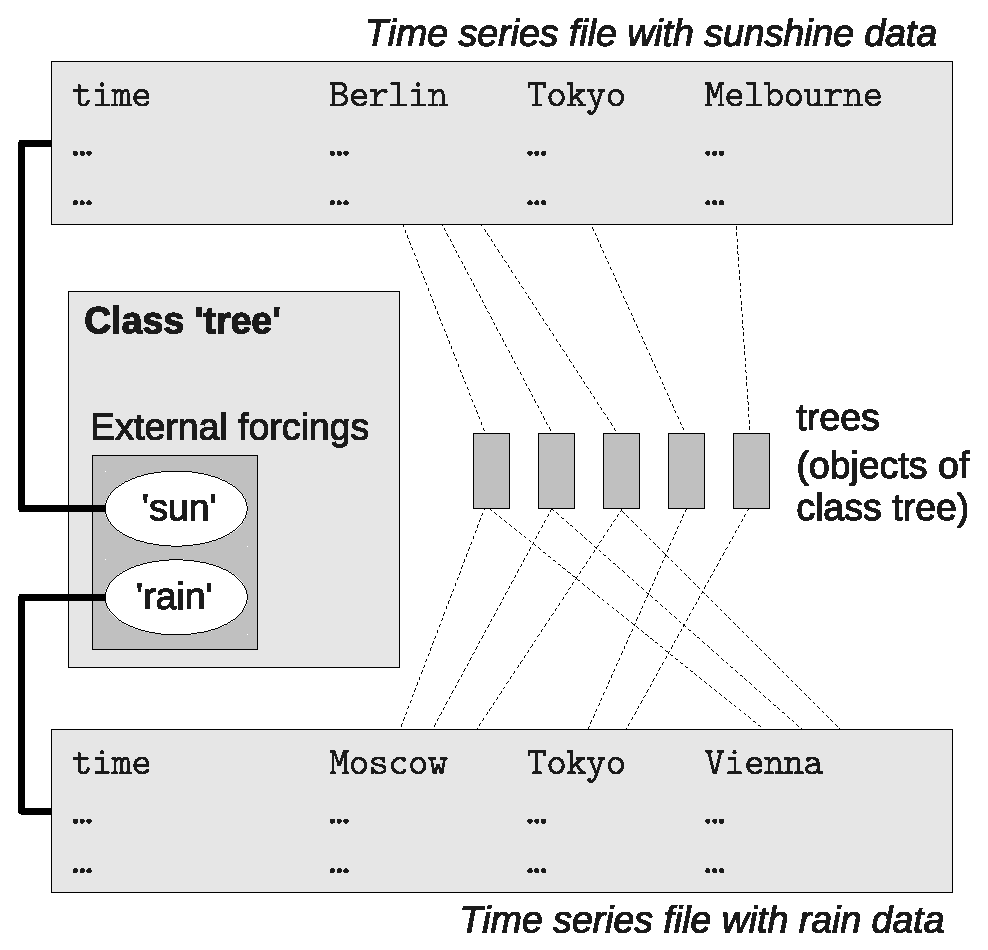
\includegraphics[width=0.9\columnwidth]{\figdir/externalForcingsManagement_overview.eps}
  \caption{Example illustrating the assignment of external forcings to objects of a particular class. \label{fig:input-external-overview}}
\end{figure}

To make this strategy work, two things have to be done:
\begin{enumerate}
  \item The two external input variables of the 'tree' class have to be linked with two time series files, containing the actual data for a single variable at all available stations. This is illustrated by the solid connecting lines in \figref{fig:input-external-overview}. The model's input file that is used to establish those links between variables and time series files is described in \secref{sec:input-externalVariables}.
  \item Links must also be established between the individual objects and the locations (\ie{} climate stations). This is illustrated by the dashed connecting lines in \figref{fig:input-external-overview}. Such links exist separately for each external forcing. Since a single object may be linked to more than one location, the links must also have a 'weight' attribute. This allows to account for the fact that Berlin is nearer to Vienna than to Moscow, when the rainfall for Berlin is estimated. The model's input file that is used to establish the links between objects and locations is described in \secref{sec:input-externalLocations}.
\end{enumerate}

%%%%%%%%%%%%%%%%%%%%%%%%%%%%%%%%%%%%%%%%%%%%%%%%%%%%%%%%%%%%%%%%%%%%%%%%%%%%%%%%
\subsection{Time series data files} \label{sec:input-timeseries}

A time series\index{time series} data file is a table with the usual header and \emph{two or more} columns. As an exception to the usual convention (see \secref{sec:input-formats}), the time information must always be present in the \emph{first} column of the table. The remaining $n$ column(s) contain the time-dependend values of the respective variable at $n$ locations. The order of these remaining columns is arbitrary since they are identified by their column names (which usually represent location names/IDs). The name of the first column containg the time information must be present but it is ignored. A reasonable name would be the abbreviation of the respective time zone, such as 'UTC'. An example of a time series data file is given in \figref{fig:input-timeseries}.

\begin{figure*}[htbp]
  \lstinputlisting[style=txt]{\figdir/example_timeseries.txt}
  \caption{Example of time series data file containing values of a variable at three locations. \label{fig:input-timeseries}}
\end{figure*}

The entries in the time column (first column), must comply with the subsequent rules:
\begin{itemize}
  \item Times must be encoded as stings in ISO 8601 format (\verb!YYYY-MM-DD hh:mm:ss!) as already described in \secref{sec:input-formats}. Due to this format, the highest possible resolution is 1 second.
  \item Any character can be used to separate date and time information (blank is a usual convention). It may even be identical with a character used to separate the table columns.
  \item The times must be in \emph{strictly} increasing order, \ie{} the latest data are expected in the file's first record and there must be no duplicate times.
  \item Regular as well as irregular time series are supported, \ie{} the time differences between neighbored records may be variable within a file. This offers the chance to use a higher resolution in periods of increased data variability and to use a low resolution when the values change slowly (or not at all). Such a strategy can save disk space and reduce the effort for reading data.
  \item The resolution, \ie{} the smallest time differences between \emph{any} neighbored records must be $\geq$ the simulation time step (see keyword \verb!delta_t! in \tabref{tab:config-time}). To give an example: If the simulation time step is 1 hour (\verb!delta_t=3600!), one can use time series with a minimum resolution of 1 hour or more (\ie{} 1 hour, 2 hours, 1 day, 3 days, etc.). A time series file containing (some/only) 5 minute data, for example, will not be accepted.
  \item If the resolution of the time series data file $\Delta t$ differs (for some or all interval(s)) from the simulation time step \verb!delta_t!, the values are automatically transformed (\ie{} reduced) if they represent sums (see discussion of column \verb!sums! in \secref{sec:input-externalVariables}).
\end{itemize}

With respect to the data values, the following restrictions apply:
\begin{itemize}
  \item The values always represent averages or sums over a certain time interval (\ie{} they do not represent instantaneous values). The respective time interval is determined by the difference in times between two neighbored records (see discussion of column \verb!past! in \secref{sec:input-externalVariables} for details).
  \item Missing values or special values used to identify invalid data (such as \verb!NA!) are \emph{not} supported. Thus, data gaps must be handled by external software (or manual work) prior to model application. It is possible, however, to use special numerical values (often -9999) to mark missing/invalid data and to treat them properly in the classes' simulate methods.
\end{itemize}

%%%%%%%%%%%%%%%%%%%%%%%%%%%%%%%%%%%%%%%%%%%%%%%%%%%%%%%%%%%%%%%%%%%%%%%%%%%%%%%%
\subsection{Assignment of time series files and attributes to variables} \label{sec:input-externalVariables}

Each external input variable\index{external input} which has been declared for a particular object class must be linked to a time series file. The time series file contains the actual data and its format is described in \secref{sec:input-timeseries}. In addition to that, a time series has further attributes which describe how the times and values are to be interpreted.

All information on the linkage of variables and time series files as well as time series attributes hast to be supplied in a single table with the following four columns:

\begin{columndef}
  \item [variable] (\textit{string}) Names of the external input variables.
  \item [file] (\textit{string}) Names of the files containing the time series data for an external input variable (see \secref{sec:input-timeseries} for details on the format and restrictions).
  \item [sums] (\textit{logical}) If \true{}, the data value related to a particular time interval is interpreted as a sum. This is appropriate for data generally measured as sums. Examples include precipitation (given in units of mm/interval) or radiation (if expressed in units of Joule/interval). If \false{}, the data are interpreted as averages over the time interval. This is appropriate, for example in case of velocities (m/s) and the like, temperatures, or radiation intensities (expressed in units of Watts).
  \item [past] (\textit{logical}) It is a common practice that time series data files contain a single time column only, even if the stored values represent averages or sums over time intervals instead of instantaneous values (see \secref{sec:input-timeseries}). Consequently, there must be a convention whether a given time marks the \emph{begin} or the \emph{end} of an interval. This is accomplished through the setting of \verb!past!. If \verb!past=true!, it is assumed that the times given in the respective column of a time series data file mark \emph{end-of-intervals}. This is a intuitive convention used by many (but not all) data providers. It is important to note that the begin of the time interval related to the very first record in the file is \emph{unknown} if \verb!past=true!. Consequently, the data values of the very first record are ignored. In contrast to that, times given in the time series file are assumed to mark the begin of time intervals, if \verb!past=false!. Then, the end of the time interval related to the last record in the file is unknown and the values are, consequently, ignored. See also \figref{fig:input-timeseries} for an example.
\end{columndef}

Note that the table does \emph{not} contain a column like \verb!objectGroup!. Thus, if an external input variable with the same name is declared in multiple object classes, the data are always taken from the same time series file. Thus, the table should contain as many records as there are unique names of external input variables in all object classes. An example of a simple table is provided in \figref{fig:input-externalVariables}.

\begin{figure*}[htbp]
  \lstinputlisting[style=txt]{\figdir/example_externalVariables.txt}
  \caption{Example of table holding information on time series data files and attributes for a set of external input variables. \label{fig:input-externalVariables}}
\end{figure*}

%%%%%%%%%%%%%%%%%%%%%%%%%%%%%%%%%%%%%%%%%%%%%%%%%%%%%%%%%%%%%%%%%%%%%%%%%%%%%%%%
\subsection{Assignment of external input locations to objects} \label{sec:input-externalLocations}

The table used to establish the links between objects and certain columns of a time series data file (that usually represent different locations) consists of the four colums described below:

\begin{columndef}
  \item [object] (\textit{string}) Names (ID strings) of objects getting external input.
  \item [variable] (\textit{string}) Names of the external input variable(s).
  \item [location] (\textit{string}) Location(s) to be assigned to a particular variable for a particular object. The used location name must be an existing column in the time series data linked to the respective variable (see \secref{sec:input-externalVariables}).
  \item [weight] (\textit{numeric}) Weights to be assigned to a particular station for a particular variable and object. If, for a specific variable, an object uses data from only a single location, the weight is generally 1.0. If, for a specific variable, the object is linked to multiple stations, the \emph{sum of weights} over all locations (for that variable) is 1.0. This is just the usual case of spatial interpolation or, more generally, weighted averaging (see \eqnref{eqn:input-externalLocationWeights}).
\end{columndef}

The value of an external forcing\index{external input} applied to a particular object at a particular time, $X$ is computed according to \eqnref{eqn:input-externalLocationWeights}. In this equation, $w_i$ is the weight of a location with index $i$ as assigned in the \verb!weight! column of the described table. The symbol $v_i$ denotes the value of the external variable for the same location (index $i$) read from the respective time series data file. The number of involved locations is $n$.

\begin{equation}
  \label{eqn:input-externalLocationWeights}
  X = \sum_{i=1}^{n} w_i \cdot v_i
\end{equation}

The described weighting approach and its typical use in the context of spatial interpolation is illustrated by \figref{fig:input-externalLocationWeights}. In the shown cases (a) and (b), the number of involved locations $n$ with respect to a particular object and variable is 1 and the assigned weight $w_1$ equals 1.0. In the cases (c) and (d) we have $n>1$ and multiple weights whose values satisfy \eqnref{eqn:input-externalLocationWeights}.

\begin{figure}[htbp]
  \centering
  \begin{tabular}{cc}
  (a) & (b) \\
  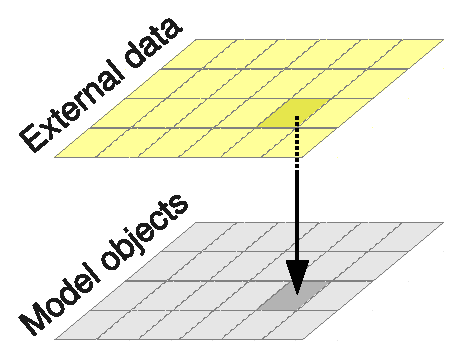
\includegraphics[width=0.45\columnwidth]{\figdir/externalinputs_weights_a.eps} &
  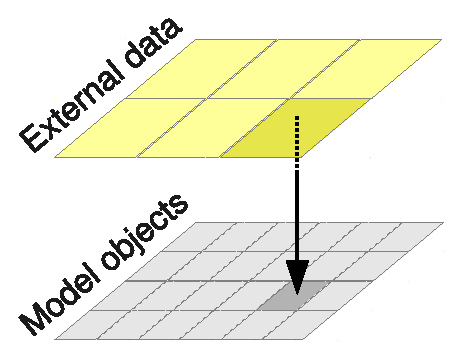
\includegraphics[width=0.45\columnwidth]{\figdir/externalinputs_weights_b.eps} \\
  (c) & (d) \\
  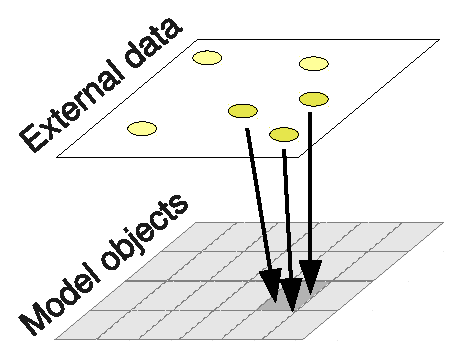
\includegraphics[width=0.45\columnwidth]{\figdir/externalinputs_weights_c.eps} &
  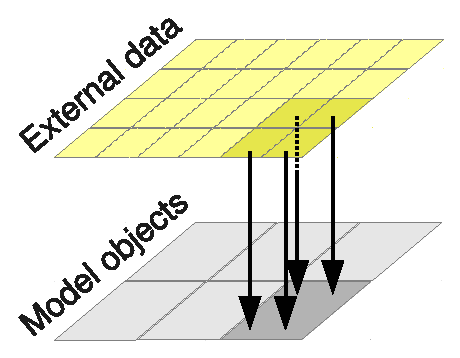
\includegraphics[width=0.45\columnwidth]{\figdir/externalinputs_weights_d.eps} \\
  \end{tabular}
  \caption[Assignment of values of an external variable measured at multiple locations to the simulated objects.]{Assignment of values of an external variable measured at multiple locations to the simulated objects (here represented by grid cells). Shown are typical situations arising in spatially distributed modeling: (a) Spatial resolution of the external variable matches with the model's resolution, (b) Use of low-resolution input in a high-resolution model, (c) Estimation of an object's input by interpolation of point data, (d) Use of high-resolution data in a low-resolution model. \label{fig:input-externalLocationWeights}}
\end{figure}

A minimum example of a table assigning external input locations to objects is given in \figref{fig:input-externalLocations}. This table corresponds to the example introduced in \secref{sec:input-external-overview}. In realistic, more complex models, such a table may become quite large, especially if many objects are simulated that use information of multiple external input variables and the input (for a specific object and variable) is taken from multiple locations. This is due to the fact that the information for all objects (of all classes) is collected in a single table.

\begin{figure*}[htbp]
  \lstinputlisting[style=txt]{\figdir/example_externalLocations.txt}
  \caption[Example of table holding information on the links between the simulated objects and the locations where data of external input variables are available.]{Example of table holding information on the links between the simulated objects and the locations where data of external input variables are available. The table corresponds to the example used in \secref{sec:input-external-overview} (\figref{fig:input-external-overview}). \label{fig:input-externalLocations}}
\end{figure*}

%%%%%%%%%%%%%%%%%%%%%%%%%%%%%%%%%%%%%%%%%%%%%%%%%%%%%%%%%%%%%%%%%%%%%%%%%%%%%%%%
%%%%%%%%%%%%%%%%%%%%%%%%%%%%%%%%%%%%%%%%%%%%%%%%%%%%%%%%%%%%%%%%%%%%%%%%%%%%%%%%
%%%%%%%%%%%%%%%%%%%%%%%%%%%%%%%%%%%%%%%%%%%%%%%%%%%%%%%%%%%%%%%%%%%%%%%%%%%%%%%%

\FloatBarrier

\section{Initialization of states} \index{state variable!initialization}

%%%%%%%%%%%%%%%%%%%%%%%%%%%%%%%%%%%%%%%%%%%%%%%%%%%%%%%%%%%%%%%%%%%%%%%%%%%%%%%%
\subsection{Initialization table for scalar states} \label{sec:input-initScal}

This table contains the initial values of all the scalar state variables of all simulated objects (see \figref{fig:input-initScal} for an example). The three required columns are defined as follows:

\begin{columndef}
  \item [object] (\textit{string}) Names (ID strings) of all objects with one or more scalar state variable(s).
  \item [variable] (\textit{string}) Names of the scalar state variable(s).
  \item [value] (\textit{numeric}) Initial values assigned to the corresponding variables of the respective models.
\end{columndef}

\begin{figure*}[htbp]
  \lstinputlisting[style=txt]{\figdir/example_initScal.txt}
  \caption{Example of table with initial values of scalar state variables. \label{fig:input-initScal}}
\end{figure*}

%%%%%%%%%%%%%%%%%%%%%%%%%%%%%%%%%%%%%%%%%%%%%%%%%%%%%%%%%%%%%%%%%%%%%%%%%%%%%%%%
\subsection{Initialization table for vector states} \label{sec:input-initVect}

As opposed to the initialization table for scalar state variables (see \secref{sec:input-initScal}), the initialization table for vector state variables has an additional column named \verb!index!. This column is of type \textit{integer} and contains the element indices corresponding to the vector state variable specified in the \verb!variable! column. The following rules apply to the \verb!index! column:
\begin{itemize}
  \item The C/C++ convention is used for the vectors' indices, \ie{} the index of a vector's first element is 0 (not 1, as in many other programming languages).
  \item For each model and variable, at least one record must be present with a value of 0 in the \verb!index! column. Thus, an initial value must be present at least for one (the first) element of each vector.
  \item More records may follow for a particular model and variable, with values of 1 through $n$ in the index column. The index values must increase by 1 from one record to the next, \ie{} there must be no gaps in the sequence of indices.
  \item The highest index value, $n$, determines the \emph{initial size} of a vector. Since indexing starts at 0, the total vector size (number of elements) is $n-1$. Note that a vector's size may change during simulation, depending on the code of the simulate method of the corresponding model class.
\end{itemize}

A simple example of an initialization table for vector state variables is given in \figref{fig:input-initVect}.

\begin{figure*}[htbp]
  \lstinputlisting[style=txt]{\figdir/example_initVect.txt}
  \caption[Layout of a table with initial values of vector state variables.]{Layout of a table with initial values of vector state variables. The example corresponds to a model of apple trees having a variable number of fruits. Consequently, all properties of the individual apples must be held in vector state variables. Initially, the apple tree 'tree1' has three fruits and 'tree2' has only two. Depending on the implementation of the apple tree class, these numbers may change during simulation.
 \label{fig:input-initVect}}
\end{figure*}

%%%%%%%%%%%%%%%%%%%%%%%%%%%%%%%%%%%%%%%%%%%%%%%%%%%%%%%%%%%%%%%%%%%%%%%%%%%%%%%%
%%%%%%%%%%%%%%%%%%%%%%%%%%%%%%%%%%%%%%%%%%%%%%%%%%%%%%%%%%%%%%%%%%%%%%%%%%%%%%%%
%%%%%%%%%%%%%%%%%%%%%%%%%%%%%%%%%%%%%%%%%%%%%%%%%%%%%%%%%%%%%%%%%%%%%%%%%%%%%%%%

\FloatBarrier

\section{Model output control} \index{output}

%%%%%%%%%%%%%%%%%%%%%%%%%%%%%%%%%%%%%%%%%%%%%%%%%%%%%%%%%%%%%%%%%%%%%%%%%%%%%%%%
\subsection{Selecting output variables for specific objects} \label{sec:input-outputSelected} \index{output!selection}

For each object, the output of simulated values in the form of time series may be requested. Note that this is restricted to those variables which have been declared as 'outputs' in the corresponding class. Consequently, if time series output for a state variable is required, for example, one must declare an (additional) output variable in the respective object class and the values of the state variable must be assigned to the output variable in each time step. The same procedure is necessary in order to output time series of an object's external inputs, functions, etc. The table used to request output of certain variables for certain objects has the following two columns:

\begin{columndef}
  \item [object] (\textit{string}) Names (ID strings) of objects for which output is requested.
  \item [variable] (\textit{string}) Names of output variables declared in the classes corresponding to the objects. A separate record is expected for each variable.
  \item [digits] (\textit{integer}) Controls the number of digits after the decimal place. Numbers are always printed in a fixed format, \ie{} as 0.33 instread of 3.3e-01, for example.
\end{columndef}

An example of such a table is given in \figref{fig:input-outputSelected}. It is important to note that it is \emph{not} checked whether the entries in the \verb!object! column actually represent the names of existing objects. Thus, to turn off \verb!any! output, one could just supply a single record with a non-existing object's name.

\begin{figure*}[htbp]
  \lstinputlisting[style=txt]{\figdir/example_outputSelected.txt}
  \caption{Example of a table used to request the writing of time series files for selected output variables of certain models.
 \label{fig:input-outputSelected}}
\end{figure*}

Also note that the time series of all variables requested for a particular object are written to a single file. The name of this file is generated automatically by appending an extension (determined by the requested format) to the object's name. The directory where the output file will appear is controlled by the value assigned to key \verb!outputDirectory! in the configuration file (see \tabref{tab:config-output}).

%%%%%%%%%%%%%%%%%%%%%%%%%%%%%%%%%%%%%%%%%%%%%%%%%%%%%%%%%%%%%%%%%%%%%%%%%%%%%%%%
\subsection{Enabling debug output for specific objects} \label{sec:input-outputDebug} \index{output!debug}

By requesting debug output for certain objects, it is possible to create time series outputs for basically \emph{all} computed values, namely
\begin{itemize}
  \item Scalar state variables
  \item Vector state variables
  \item External input variables
  \item Simulated input variables
  \item Output variables.
\end{itemize}

This kind of output is particularly useful when debugging a model. Depending on the complexity of an object's data and the number of simulated time steps, the produced output files may become quite large. Therefore, the approach described in \secref{sec:input-outputSelected} is usually more appropriate if only some of the computed quantities are actually of interest.

The table used to request debug outputs consists of just a single column with name \verb!object! (no example given). It holds the names (ID strings) of the objects for which output is requested. It is \emph{not} checked whether the entries in that column represent the names of existing objects. Thus, if no debug output is required at all, the table should contain just a single record with a non-existing object's name. Note that the writing of large debug output files that are not actually required may lead to a significant waste of computing time and disk space.

The name(s) of the output file(s) are generated automatically by appending an extension (currently \texttt{.dbg}) to the objects' name(s). The directory where the output files will appear is controlled by the value assigned to key \verb!outputDirectory! in the configuration file (see \tabref{tab:config-output}).

%%%%%%%%%%%%%%%%%%%%%%%%%%%%%%%%%%%%%%%%%%%%%%%%%%%%%%%%%%%%%%%%%%%%%%%%%%%%%%%%
\subsection{Output of the model's state at selected times}  \label{sec:input-outputState} \index{output!model state}

In some situation is is desirable to write the values of all state variables of all simulated \emph{at a certain point in time} to disk. Potential uses of the produced file(s) containing the \emph{entire model's state} include
\begin{itemize}
  \item restarting of the model, using the produced files to initialize the state variables in a subsequent call,
  \item visualization of spatial patterns.
\end{itemize}

The table used to request outputs of the model's state consists of just a single column with name \verb!time! (no example given). It holds the times for which the output is requested as strings in the usual ISO 8601 format (see \secref{sec:input-formats}). One should note that output is only created if a specified time also represents the end of a simulation time step (exactly to the second). Thus, it is not possible to request the model's state for intermediate times (such as 07:30, if the simulation time step is 1 hour and the model was started at a full hour).
The only technique of suppressing outputs of the model's state at all is to specify (valid) times that do not meet the above criteria. Preferably, one specifies just a single time which is far outside the simulation time window and easily identified as a dummy such as \verb!1900-01-01 00:00:00!, for example. Saving state information for many time steps despite of the fact that it is not actually required wastes both computing time and disk space.

For each point in time, two output files are created. One of the files contains the current values of scalar state variables and the other file holds the values of the vector state variables. The used formats are identical to the initialization tables described in \secref{sec:input-initScal} (\figref{fig:input-initScal}) and \secref{sec:input-initVect} (\figref{fig:input-initVect}), respectively.

The name(s) of the output file(s) are generated automatically using the respective time stamp. The values of the scalar state variables are saved in file \verb!statesScal_YYYYMMDDhhmmss! and the vector state variables are written to file \verb!statesVect_YYYYMMDDhhmmss!.The 14 digits at the end of the file names encode the time (4-digit year, followed by 2-digit month, day, hour, minute, and second). The directory where the output files will appear is controlled by the value assigned to key \verb!outputDirectory! in the configuration file (see \tabref{tab:config-output}).

%%%%%%%%%%%%%%%%%%%%%%%%%%%%%%%%%%%%%%%%%%%%%%%%%%%%%%%%%%%%%%%%%%%%%%%%%%%%%%%%
\subsection{Precision of printed outputs}  \label{sec:input-outputPrecision} \index{output!precision}

The current version of the \software{echse} writes all output data in a scientific format with three digits after the period. Thus, numbers are formatted like \texttt{$\pm$X.YYYe$\pm$ZZ}, where \texttt{ZZ} is the exponent (base 10) corresponding to the number \texttt{X.YYY}. Currently, the output format \emph{cannot} be changed by the model user.

A potential issue with the \texttt{$\pm$X.YYYe$\pm$ZZ} format is that the precision of output data is limited to a total number of 4 digits. This is sufficient for many applications but may sometimes be problematic. In such cases, it is recommended to transform the data by adding or subtracting an appropriate constant (at latest before calling the \verb!set_output()! method; see \tabref{tab:concept-dataAccessFunctions_write}).

Let's consider the example of a reservoir in a mountainous region. Suppose that the reservoir's water level ranges from 2150 to 2180 m (a.s.l.) due to operation and fluctuations of the inflow. If the model writes the simulated water level to output files in units of m a.s.l., the precision is limited to 1~m only! To notice that, one must consider that the minimum and maximum values would be printed as \texttt{2.150e+03} and \texttt{2.180e+03}, respectively. By subtracting an appropriate constant, say 2100, the output precision can be increased significantly because the new data range is 50--80 (printed as \texttt{5.000e+01} and \texttt{8.000e+01}, respectively). After the transformation, the precision of the printed data is about 1~cm, \ie{} 100 times higher.
